\newcommand\xsetpos{3}
\definecolor{myblue}{RGB}{56,94,101}
\definecolor{myturq}{RGB}{173, 234, 234}

\begin{figure}
   \begin{subfigure}{0.49\textwidth}
      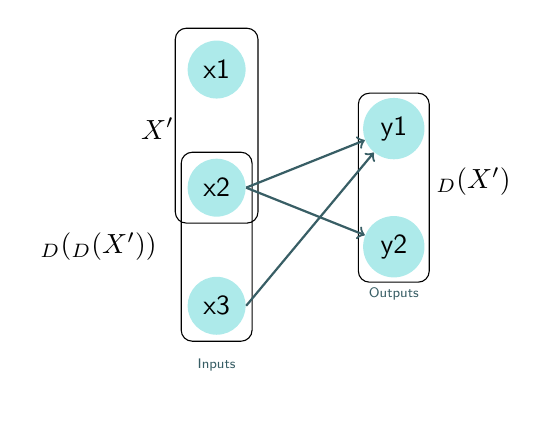
\begin{tikzpicture}[scale=.75,
               arrow/.style={thick,->,myblue},
               set name/.style={font=\color{myblue}\tiny\bfseries\sf},
               set/.style={ultra thick,myblue},
               every node/.style={circle},
               font=\sf
            ]
         % \draw[set] (0,0) rectangle ++(1, 2)
         %      (\xsetpos,0) rectangle ++(1, 2);
         \node[set name] at (0.5, -2.5) {Inputs};
         \node[set name] at (3.5, -1.3) {Outputs};

         \node (X') at (-0.5, 1.5) {$X'$};
         \node (X'') at (-1.5, -0.5) {$\demandR_{D}(\demandByR_D(X'))$};
         \node (DX') at (4.85, 0.6) {$\demandByR_D(X')$}; 
         \node[fill=myturq] (x1) at (0.5, 2.5) {x1};
         \node[fill=myturq] (x2) at (0.5, 0.5) {x2};
         \node[fill=myturq] (x3) at (0.5, -1.5) {x3};
         \node[fill=myturq] (y1) at (3.5, 1.5) {y1};
         \node[fill=myturq] (y2) at (3.5, -0.5) {y2};
         \draw[rounded corners] (-0.1, 1.1) rectangle (1.1, -2.1);
         \draw[rounded corners] (-0.2, 3.2) rectangle (1.2, -0.1);
         \draw[rounded corners] (2.9, 2.1) rectangle (4.1, -1.1);
         \begin{scope}[arrow]
            \draw (x2.east) -- (y1);
            \draw (x2.east) -- (y2);
            \draw (x3.east) -- (y1);
         \end{scope}
      \end{tikzpicture}
      \caption{Round-trip grows}
      \label{fig:relation-not-galois-1}
   \end{subfigure}
   \hfill
   \begin{subfigure}{0.49\textwidth}
      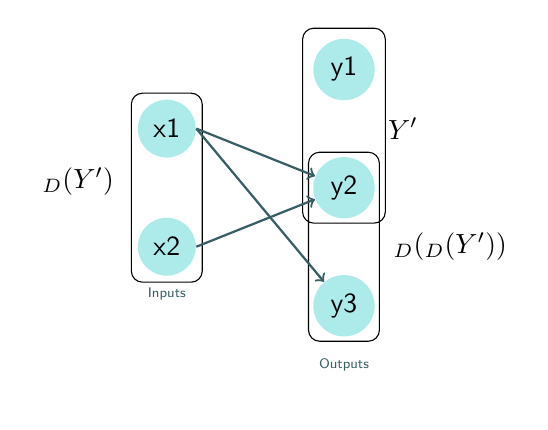
\begin{tikzpicture}[scale=.75,
               arrow/.style={thick,->,myblue},
               set name/.style={font=\color{myblue}\tiny\bfseries\sf},
               set/.style={ultra thick,myblue},
               every node/.style={circle},
               font=\sf
            ]
         % \draw[set] (0,0) rectangle ++(1, 2)
         %      (\xsetpos,0) rectangle ++(1, 2);
         \node[set name] at (0.5, -1.3) {Inputs};
         \node[set name] at (3.5, -2.5) {Outputs};

         \node (Y') at (4.5, 1.5) {$Y'$};
         \node (Y'') at (5.3, -0.5) {$\demandByR_{D}(\demandR_D(Y'))$};
         \node (DY') at (-1.0, 0.6) {$\demandR_D(Y')$}; 
         \node[fill=myturq] (y1) at (3.5, 2.5) {y1};
         \node[fill=myturq] (y2) at (3.5, 0.5) {y2};
         \node[fill=myturq] (y3) at (3.5, -1.5) {y3};
         \node[fill=myturq] (x1) at (0.5, 1.5) {x1};
         \node[fill=myturq] (x2) at (0.5, -0.5) {x2};
         \draw[rounded corners] (2.9, 1.1) rectangle (4.1, -2.1);
         \draw[rounded corners] (2.8, 3.2) rectangle (4.2, -0.1);
         \draw[rounded corners] (-0.1, 2.1) rectangle (1.1, -1.1);
         \begin{scope}[arrow]
            \draw (x1.east) -- (y2);
            \draw (x1.east) -- (y3);
            \draw (x2.east) -- (y2);
         \end{scope}
      \end{tikzpicture}
      \caption{Round trip shrinks}
      \label{fig:relation-not-galois-2}   
   \end{subfigure}
   \caption{In \figref{relation-not-galois-1}, the round trip grows, and in \figref{relation-not-galois-2},
   it shrinks, contradicting a property of Galois connections. \todo{We should potentially extend this
   diagram from the other direction, to show the lack of monotonicity in the presence of free outputs}}
   \label{fig:relation-not-galois}
\end{figure}